% SC1007 — Chapter 4: BST, AVL & Red-Black Sketch
% No \documentclass — included by modules/SC1007/main.tex (book class).
\chapter{Binary Search Trees \& Balanced Trees}
\label{ch:bst-balanced}

\begin{quote}
\emph{``A sorted tree is a sorted array you can grow.''} --- But only if it stays balanced.
\end{quote}

\noindent\textbf{Prerequisites:} Ch.~3 (trees, traversals). BST is the bridge from trees to ordered dictionaries; AVL/red-black keep it $O(\log n)$.

\section*{Learning Outcomes}
After this chapter you will be able to:
\begin{enumerate}[label=(L\arabic*)]
    \item maintain the BST invariant and implement search/insert/delete in $O(h)$;
    \item explain why worst-case $h=\Theta(n)$ and how balancing fixes it;
    \item perform AVL rotations and verify the AVL balance invariant;
    \item sketch red-black invariants and argue $O(\log n)$ height.
\end{enumerate}

% ============================================================
\section{Binary Search Trees}
\label{sec:bst}

\begin{definition}[BST invariant]
For every node $v$, all keys in $v.\text{left}$ are $<v.\text{key}$ and all keys in $v.\text{right}$ are $>v.\text{key}$ (assume distinct keys).
\end{definition}

Consequence: inorder traversal yields keys in sorted order (Ch.~3).

\begin{figure}[h]
\centering
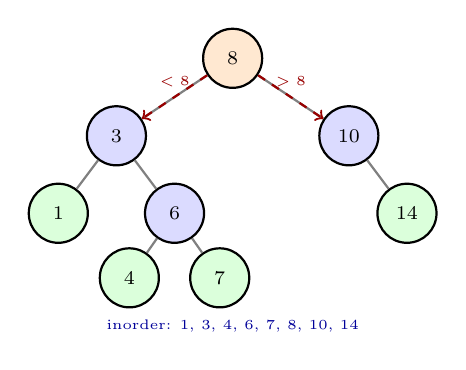
\begin{tikzpicture}[scale=0.82, every node/.style={font=\scriptsize},
  tnode/.style={circle, draw, thick, fill=blue!14, minimum size=0.75cm},
  edge/.style={thick, black!50}]
  \node[tnode, fill=orange!18] (8) at (3,2.4) {8};
  \node[tnode] (3) at (1.2,1.2) {3};
  \node[tnode] (10) at (4.8,1.2) {10};
  \node[tnode, fill=green!14] (1) at (0.3,0) {1};
  \node[tnode] (6) at (2.1,0) {6};
  \node[tnode, fill=green!14] (14) at (5.7,0) {14};
  \node[tnode, fill=green!14] (4) at (1.4, -1.0) {4};
  \node[tnode, fill=green!14] (7) at (2.8, -1.0) {7};
  \draw[edge] (8)--(3); \draw[edge] (8)--(10); \draw[edge] (3)--(1); \draw[edge] (3)--(6);
  \draw[edge] (6)--(4); \draw[edge] (6)--(7); \draw[edge] (10)--(14);
  % BST range annotations
  \node[font=\tiny, blue!60!black] at (3,-1.75) {inorder: 1, 3, 4, 6, 7, 8, 10, 14};
  \draw[->, red!60!black, thick, dashed] (8) -- (3) node[midway, above, font=\tiny] {$<8$};
  \draw[->, red!60!black, thick, dashed] (8) -- (10) node[midway, above, font=\tiny] {$>8$};
\end{tikzpicture}
\caption{A BST. Every left subtree holds smaller keys, every right subtree larger. Inorder is sorted.}
\label{fig:bst-example}
\end{figure}

Operations (all $O(h)$ where $h$ is height):

\begin{lstlisting}[language=Python]
def search(root, k):
    while root and root.key != k:
        root = root.left if k < root.key else root.right
    return root  # None if absent

def insert(root, k):
    if not root: return Node(k)
    if k < root.key:  root.left  = insert(root.left, k)
    elif k > root.key: root.right = insert(root.right, k)
    return root

def delete(root, k):  # three cases: leaf / one child / two children
    if not root: return None
    if k < root.key:  root.left  = delete(root.left, k)
    elif k > root.key: root.right = delete(root.right, k)
    else:  # found
        if not root.left:  return root.right
        if not root.right: return root.left
        # two children: replace with successor
        succ = min_node(root.right)
        root.key = succ.key
        root.right = delete(root.right, succ.key)
    return root
\end{lstlisting}

Successor $=$ minimum in right subtree (leftmost descendant). All ops follow one root-to-leaf path: $O(h)$ time, $O(h)$ stack space.

\textbf{Degeneracy.} Inserting sorted keys $1,2,3,\ldots,n$ yields a chain with $h=n-1$: every operation degrades to $\Theta(n)$. Balanced trees prevent this.

% ============================================================
\section{AVL Trees}
\label{sec:avl}
AVL (Adelson-Velsky--Landis, 1962) maintains the \emph{AVL invariant}: for every node,
\begin{equation}
|\,\text{height}(\text{left}) - \text{height}(\text{right})\,| \le 1.
\label{eq:avl-invariant}
\end{equation}
This forces $h=\Theta(\log n)$ (Fibonacci bound: $n\ge F_{h+2}-1$, so $h\le1.44\log_{2}n$).

\textbf{Rebalancing via rotations.} After insertion/deletion, walk up updating heights; at the first unbalanced node, apply one of four rotations:

\begin{figure}[h]
\centering
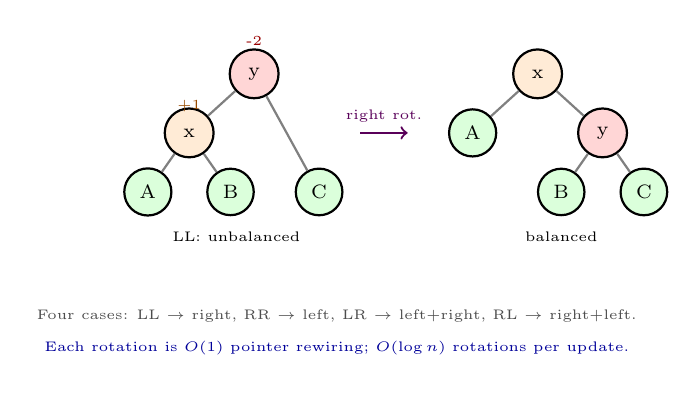
\begin{tikzpicture}[scale=0.75, every node/.style={font=\scriptsize},
  tnode/.style={circle, draw, thick, fill=blue!14, minimum size=0.62cm},
  edge/.style={thick, black!50}]
  % Left-Left case: right rotation
  \begin{scope}
    \node[tnode, fill=red!16] (y) at (1.8,1.6) {y};
    \node[tnode, fill=orange!16] (x) at (0.7,0.6) {x};
    \node[tnode, fill=green!14, minimum size=0.50cm] (a) at (0.0,-0.4) {A};
    \node[tnode, fill=green!14, minimum size=0.50cm] (b) at (1.4,-0.4) {B};
    \node[tnode, fill=green!14, minimum size=0.50cm] (c) at (2.9,-0.4) {C};
    \draw[edge] (y)--(x); \draw[edge] (y)--(c); \draw[edge] (x)--(a); \draw[edge] (x)--(b);
    \node[font=\tiny, red!60!black] at (1.8,2.15) {-2};
    \node[font=\tiny, orange!60!black] at (0.7,1.05) {+1};
    \node at (1.5,-1.15) {\tiny LL: unbalanced};
  \end{scope}
  \draw[->, thick, violet!70!black] (3.6,0.6) -- (4.4,0.6) node[midway, above, font=\tiny] {right rot.};
  \begin{scope}[xshift=5.5cm]
    \node[tnode, fill=orange!16] (xp) at (1.1,1.6) {x};
    \node[tnode, fill=green!14, minimum size=0.50cm] (ap) at (0.0,0.6) {A};
    \node[tnode, fill=red!16] (yp) at (2.2,0.6) {y};
    \node[tnode, fill=green!14, minimum size=0.50cm] (bp) at (1.5,-0.4) {B};
    \node[tnode, fill=green!14, minimum size=0.50cm] (cp) at (2.9,-0.4) {C};
    \draw[edge] (xp)--(ap); \draw[edge] (xp)--(yp); \draw[edge] (yp)--(bp); \draw[edge] (yp)--(cp);
    \node at (1.5,-1.15) {\tiny balanced};
  \end{scope}
  % Second row: LR case hint
  \begin{scope}[yshift=-2.8cm, xshift=1.2cm]
    \node[font=\tiny, gray!60!black] at (2.0,0.3) {Four cases: LL $\to$ right, RR $\to$ left, LR $\to$ left+right, RL $\to$ right+left.};
    \node[font=\tiny, blue!60!black] at (2.0,-0.25) {Each rotation is $O(1)$ pointer rewiring; $O(\log n)$ rotations per update.};
  \end{scope}
\end{tikzpicture}
\caption{AVL right rotation for the LL case (left child too tall). The other three cases are symmetric. After rotation, heights of $x,y$ are recomputed and the invariant is restored.}
\label{fig:avl-rotation}
\end{figure}

\begin{figure}[h]
\centering
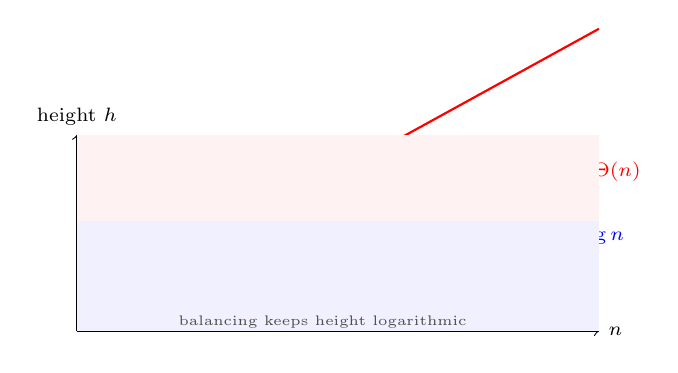
\begin{tikzpicture}[scale=0.78, every node/.style={font=\scriptsize}]
  \draw[->] (0,0) -- (8.5,0) node[right] {$n$};
  \draw[->] (0,0) -- (0,3.2) node[above] {height $h$};
  \draw[red, thick] plot[domain=0.2:8.5, smooth] (\x,{0.25+0.55*\x});
  \node[red] at (7.5,2.6) {unbalanced $h=\Theta(n)$};
  \draw[blue, thick] plot[domain=0.3:8.5, smooth] (\x,{0.25+0.65*ln(\x+1)/ln(2)});
  \node[blue] at (7.5,1.55) {AVL $h\le1.44\lg n$};
  \fill[red!5] (0,1.8) rectangle (8.5,3.2);
  \fill[blue!6] (0,0) rectangle (8.5,1.8);
  \node[font=\tiny, gray!60!black] at (4,0.15) {balancing keeps height logarithmic};
\end{tikzpicture}
\caption{Height comparison: unbalanced BST can be linear; AVL guarantees logarithmic height.}
\label{fig:avl-height}
\end{figure}

Insert/delete may need $O(\log n)$ rotations walking to root, but each rotation is $O(1)$.

% ============================================================
\section{Red-Black Trees (Sketch)}
\label{sec:red-black}
Red-black trees relax the AVL condition for fewer rotations. Each node is coloured red or black with invariants: (i) root black, (ii) no two reds adjacent, (iii) every root-to-leaf path has same number of black nodes (black-height). These imply $h\le2\log_{2}(n+1)$.

Insertion colours the new node red, then fixes violations by recolouring and at most two rotations along the path. STL \texttt{map}/\texttt{set} (C++) and Java \texttt{TreeMap} are typically red-black trees.

AVL is more strictly balanced (faster lookups); red-black has fewer rotations on updates (faster insertions). Both are $O(\log n)$ worst-case.

% ============================================================

% --- Additional: BST analysis and rotations in detail ---
\section{Analysis \& Rotation Details}
\label{sec:bst-analysis}
\textbf{Search cost $=\,h+1$ comparisons.} In a random BST built from random insertions, expected $h=\Theta(\log n)$; worst-case $h=n-1$ (sorted input). This motivates self-balancing.

\textbf{Rotations preserve inorder.} A right rotation at $y$ with left child $x$:
\begin{equation}
\text{inorder}(y\text{ subtree before}) = A,x,B,y,C = \text{inorder}(x\text{ subtree after}),
\end{equation}
where $A,B,C$ are subtrees. Only $O(1)$ pointers change; heights of $x,y$ are recomputed. Left rotation is symmetric; LR $=$ left on $x$ then right on $y$.

\begin{lstlisting}[language=Python]
# Right rotation at y (y.left == x) -- O(1)
def rotate_right(y):
    x = y.left
    y.left = x.right
    x.right = y
    update_height(y); update_height(x)
    return x  # new subtree root
\end{lstlisting}

\begin{remark}
Red-black insertion needs at most 2 rotations; AVL may need $O(\log n)$ up the path. Hence red-black is preferred when insertions dominate, AVL when lookups dominate.
\end{remark}

\section{Chapter Notes}
CLRS Ch.~12--13, Weiss Ch.~4.2--4.3. AVL Fibonacci bound proof by induction on height.

% ============================================================
\section{Exercises}
\label{sec:ch04-exercises}
\begin{enumerate}[label=E4.\arabic*, leftmargin=*, itemsep=0.7em]
    \item \textbf{BST ops.} Insert $8,3,10,1,6,14,4,7$ into empty BST in order. Draw the tree after each insertion and list inorder. Delete $3$ (two children) and show the successor replacement.
    \item \textbf{AVL insertion.} Insert $1,2,3,4,5,6$ into empty AVL. Show rotations at each step and verify Eq.~\eqref{eq:avl-invariant} holds.
    \item \textbf{Height bound.} Prove $n\ge F_{h+2}-1$ for AVL of height $h$ ($F_{k}$ Fibonacci). Deduce $h\le1.44\log_{2}n$.
    \item \textbf{Red-black.} Insert $10,20,30,15$ into empty red-black tree. Show colourings and rotations. Verify all three invariants after each insert.
    \item \textbf{Comparison.} Give a sequence where AVL does asymptotically more rotations than red-black on the same insertions, and explain why.
\end{enumerate}
% End of Chapter 4
